\section{NOVA}
\label{sec:nova}

NOVA fits the transmission spectrum directly to the detector pixels. One
forward model predicts the count rate of every fitted pixel as starlight,
dimmed by the transit, plus background, so the split between the two is
decided in the same fit as the transit. The fit estimates four things
together: the spectrum $D(\lambda)$, the limb darkening $\bm{u}(\lambda)$, the
brightness of the star in each detector column and the background. Everything
else is held fixed during the fit. The spatial profile, the reference spectrum
of the star, a slow curvature of the baseline, the time pattern of the
background, a noise scale for each pixel and the orbital geometry are
estimated beforehand from each input. The depth bins, the limb-darkening
reference, the apertures, the off-trace pixels, the background maps and two
noise scales are the same for every input.

In this section, I describe NOVA as it is currently implemented, and end with a
first, preliminary spectrum of the real WASP-17~b visit.

\subsection{Detector processing}
\label{sec:detector-processing}

NOVA's input is prepared from the raw ramps with the JWST calibration pipeline
\citep{JWSTPipeline2025} and exoTEDRF \citep{Radica2024}. The JWST group steps
run up to and including the reference-pixel correction. exoTEDRF then removes
the $1/f$ noise once from each group, by subtracting the median of each column
outside the trace cores. For this step only, it subtracts a scaled background
model from the groups beforehand and adds it back afterwards. Field stars found
in the F277W exposure are left out of the medians. The linearity,
jump-detection, ramp-fitting and gain steps then give count rates. Stage~2 of
exoTEDRF applies the flat field, subtracts the scaled zodiacal background model
and corrects bad pixels. I apply no further mask to the scene.

\subsection{The detector forward model}
\label{sec:forward}

\begin{figure}[t]
  \centering
  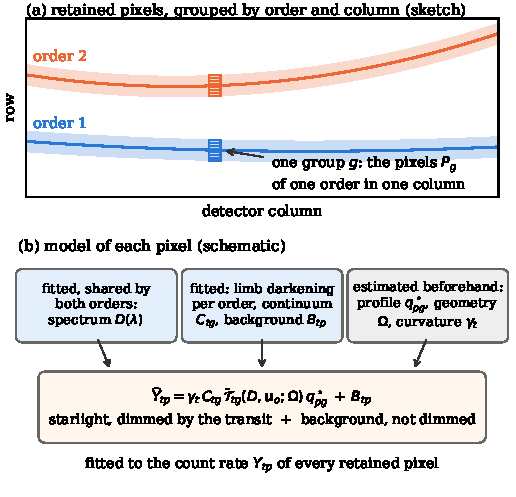
\includegraphics[width=\columnwidth]{figures/nova_schematic.pdf}
  \caption{Schematic of the detector forward model of \nova{}. (a) The
  fitted pixels are grouped by order and column (a sketch, not data), and the
  two orders do not overlap. (b) The count rate of each pixel is modelled as
  starlight, dimmed by the transit, plus a background that is not dimmed. The
  spectrum is shared by both orders, whilst the limb darkening is fitted for
  each order as penalised deviations from a theoretical reference.}
  \label{fig:nova-schematic}
\end{figure}

Within one detector column, the pixels of a trace see nearly the same
wavelength. NOVA therefore groups the pixels by order and column: each group
$g$ holds the pixels $P_g$ of one order in one column
(Figure~\ref{fig:nova-schematic}). The fitted pixels lie in two fixed
apertures along the traces. Four edge columns, the 51 reddest columns of
order~1, which the wavelength calibration does not directly cover, and flagged samples
are left out. For the count rate $Y_{tp}$ of pixel $p$ in integration $t$,
NOVA predicts
\begin{equation}
 \widehat Y_{tp}
 = \gamma_t\, C_{tg}\, \bar{\mathcal{T}}_{tp}\, \tilde q_{pg} + B_{tp},
 \label{eq:nova-forward}
\end{equation}
where $C_{tg}$ is the brightness of the star in the group $g$ of pixel $p$ at
time $t$, $\tilde q_{pg}$ is the share of that light that falls on pixel $p$
(Section~\ref{sec:response}), $\bar{\mathcal{T}}_{tp}$ is the dimming of
pixel $p$ by the transit, $\gamma_t$ is a small, fixed curvature of the
baseline (Section~\ref{sec:continuum}) and $B_{tp}$ is the background left
after Stage~2. Only the starlight is dimmed. Light assigned to the background
is not.

Which wavelengths reach which pixel is described by the response $R_{p\lambda}$,
the count rate in pixel $p$ per unit stellar flux at wavelength $\lambda$. It
contains the line-spread kernel, which spreads the light of one wavelength over
a few neighbouring columns. NOVA builds $R_{p\lambda}$ for each input with
ATOCA, the SOSS extraction code of the JWST pipeline
\citep{DarveauBernierEtAl2022,JWSTPipeline2025}, from the public trace and
wavelength calibration \citep{BainesEtAl2023Trace,BainesEtAl2023Wavelength},
kernel and throughput, with its own spatial profile $q^\star_{pg}$ in place of
the public one. The response factorises as
$R_{p\lambda}=q^\star_{pg}K_{p\lambda}$, where $K_{p\lambda}$ is the light of
wavelength $\lambda$ that reaches pixel $p$ per unit profile. Each pixel
receives the light of its own order only. The transit factor of a pixel is the
transit model $\mathcal{T}_t(\lambda)$ averaged over the light that reaches
it,
\begin{equation}
 \bar{\mathcal{T}}_{tp}
 = \frac{\sum_{\lambda} K_{p\lambda}\, s_\lambda\, \mathcal{T}_t(\lambda)}
        {\sum_{\lambda} K_{p\lambda}\, s_\lambda},
 \label{eq:pixel-transit}
\end{equation}
where $s_\lambda$ is a reference spectrum of the star, fitted to the
out-of-transit data of each input and then held fixed. The transit model
$\mathcal{T}_t(\lambda)$ depends on the depth $D$ of the bin that contains
$\lambda$, the limb darkening $\bm{u}$ of the order and the orbital state
$\Omega$. Because each pixel sees a mix of nearby wavelengths, the fitted
depths account for the line-spread kernel.

\subsection{The shared spectrum and transit model}

A planet has one transmission spectrum, whichever order records its light, so
both orders share $D(\lambda)$. It is represented by $K=160$ top-hat bins from
0.62 to $2.84\,\mu\mathrm{m}$. The bins have a target width of
$0.01\,\mu\mathrm{m}$ below $2\,\mu\mathrm{m}$ and $0.04\,\mu\mathrm{m}$
above, and each range is divided into equal bins close to that width, 0.0097
to $0.0100\,\mu\mathrm{m}$ and $0.0382\,\mu\mathrm{m}$. The bluest bin is twice
as wide, because the bin next to it received no light and was merged into it.
The two reddest bins, above $2.764\,\mu\mathrm{m}$, receive no light in the
model. Order~2 does not reach them, and order~1 is cut at
$2.758\,\mu\mathrm{m}$, beyond which the public PASTASOSS wavelength
calibration would have to be extrapolated. These two bins are held at the
white-light depth and not reported. The other 158 bins form the set $I$, and
their depths are
\begin{equation}
  D_j = \bar D\,
  \frac{\exp(h_j)}{\sum_{k\in I} w_k \exp(h_k)}, \qquad \bm{h}=\bm{H}\bm{z},
  \qquad j\in I,
  \label{eq:depth-basis}
\end{equation}
where $\bar D$ is the overall, achromatic depth level and $w_k$ are the bin
widths, normalised to sum to one over $I$. With these weights, the
width-weighted mean of the depths equals $\bar D$, and the exponential keeps
every depth positive. The vector $\bm{h}$ carries the shape of the spectrum.
Adding the same constant to every $h_j$ would not change the depths, so the
data cannot fix that direction. The fixed $158\times157$ matrix $\bm{H}$
removes it: its columns are orthonormal and each sums to zero, so
$\bm{h}=\bm{H}\bm{z}$ never contains a constant. I build $\bm{H}$ from a QR
decomposition of a vector of ones. The fitted values are only $\bar D$ and the
157 shape coordinates $\bm{z}$.

The orbital state $\Omega$ is a circular orbit with the period of
\citet{LouieEtAl2025}, and with the mid-transit time $t_0$, scaled semi-major
axis $a/R_\star$ and impact parameter $b$ from NOVA's white-light fit
(Section~\ref{sec:own-white}). The transit $\mathcal{T}_t$ is computed with
jaxoplanet \citep{Jaxoplanet2025} and averaged over each integration.

The limb darkening follows the quadratic law \citep{MandelAgol2002}, written
in the coordinates $q_1,q_2\in[0,1]$ of \citet{Kipping2013},
\begin{equation}
 u_1=2\sqrt{q_1}\,q_2, \qquad
 u_2=\sqrt{q_1}\,(1-2q_2).
 \label{eq:kipping-coordinates}
\end{equation}
Limb darkening and depth are partly degenerate, so the spectral fit lets the
limb darkening deviate only smoothly from a reference computed from STAGGER
model intensities \citep{MagicEtAl2015}. For each order and for each of $q_1$
and $q_2$, the deviation is a straight line in log-wavelength, an offset plus a
slope, so eight numbers in total. It is added to the logit of $q$,
$\ln[q/(1-q)]$, which keeps $q$ between 0 and 1 for any deviation. A straight
line in log-wavelength changes by the same amount for each factor in
wavelength, so it treats the blue and red ends of order~1, which span a factor
of 3.3, equally. Two penalties keep the deviation small: one for departing from
the reference, and one for its curvature in wavelength, which here restrains
the slope. The white-light fit, by contrast, leaves $u_1$ and $u_2$ free for
each order, with uniform priors from 0 to 1 (Section~\ref{sec:own-white}).

\subsection{The spatial profile}
\label{sec:response}

The spatial profile $q^\star_{pg}$ is the share of a column's starlight that
falls on each of its pixels, and NOVA measures it from the data. The starlight
dims during the transit and the background does not. The part of a pixel's
time series that follows the transit therefore measures its starlight,
provided that only starlight varies like the transit.

For each order $o$, I first measure the shape of the transit, $\phi_o(t)$,
directly from the pixels. At each integration, it is the median fractional
change of the brightest 65\% of the order's pixels, relative to each pixel's
out-of-transit level. A straight line in time is removed, and the curve is
scaled so that its deepest point is $-1$. Every pixel is then fitted, with
Huber weights, as
\begin{equation}
 Y_{tp} = A_{pg}\,\phi_{o}(t) + \ell_p + \kappa_p\,\tau_t + \varepsilon_{tp},
 \label{eq:qstar-fit}
\end{equation}
where $A_{pg}$ is the part of the signal that follows the transit,
$\ell_p+\kappa_p\tau_t$ is a straight line in the time $\tau_t$ and
$\varepsilon_{tp}$ is the residual. The profile is
$q^\star_{pg}=A_{pg}/\sum_{p'\in P_g}A_{p'g}$. The depth, nearly the same for
all pixels of a column, cancels in this ratio, and so does the scale of
$\phi_o$. Each amplitude rests on a dip of only 1.5 to 2\%, so I smooth the
profile across neighbouring columns, with a strength chosen by
cross-validation between alternate integrations.

The share in equation~(\ref{eq:nova-forward}) weights the profile by the
starlight that reaches each pixel,
\begin{equation}
 \tilde q_{pg} = \frac{q^\star_{pg}\, S_p}{\sum_{p'\in P_g} q^\star_{p'g}\, S_{p'}},
 \qquad S_p=\sum_\lambda K_{p\lambda}\, s_\lambda .
 \label{eq:qtilde}
\end{equation}
Because the trace is slightly tilted on the detector, the pixels of one column
see slightly different wavelengths, so $S_p$ varies a little within a column.
If it did not, $\tilde q_{pg}$ would equal $q^\star_{pg}$, and
$\bar{\mathcal{T}}_{tp}$ would be the same for every pixel of the column.

\subsection{The continuum, the background and the noise}
\label{sec:continuum}

The brightness of the star in each group is a straight line in time,
$C_{tg}=\beta_{0g}+\beta_{1g}\tau_t$, and both coefficients are fitted. The
baseline can also curve slowly, and $\gamma_t$ describes this curvature. It is
measured beforehand and held fixed. For each order, I fit a parabola in time to
the background-subtracted out-of-transit trace flux and divide it by a straight
line fitted to the same data. $\gamma_t$ is the geometric mean of the two
orders' ratios, normalised to a mean of one out of transit. It is used only if
it agrees between alternate out-of-transit integrations and stays within 0.1\%
of one. Its uncertainty is not propagated.

The curvature is kept out of $C_{tg}$ for a reason. The transit lies between
the two out-of-transit windows, where a parabola in time bulges most. A free
curvature in each column would therefore trade against that column's depth. A
single curvature, measured outside the transit and shared by all columns,
cannot.

The background is a sum of eight fixed spatial maps $\Phi_{pk}$. Each map has
a constant amplitude $\alpha_{k0}$ and an amplitude $\alpha_{k1}$ that follows
a time pattern $G_1(t)$,
\begin{equation}
 B_{tp}=\sum_{k=1}^{8}\Phi_{pk}
 \left[\alpha_{k0}+\alpha_{k1}\,G_1(t)\right].
 \label{eq:background-model}
\end{equation}
The first map is the zodiacal-light model that Stage~2 scaled and subtracted.
It is one image from a library of such models in the JWST calibration
reference file \texttt{jwst\_niriss\_bkg\_0033}. The other seven are smooth
polynomials in detector position, $1$, $y$, $x$, $xy$, $y^2$, $x^2$ and
$xy^2$, which follow large-scale gradients. All eight are made orthonormal over
the off-trace pixels. These are 244,657 pixels more than about 30 rows from
the traces, clear of field stars, bad pixels and the detector edges. The maps
and the off-trace pixels were chosen once, from the out-of-transit data of the
WASP-17 visit, and are reused for every input. Eight maps predicted held-out,
trace-shaped strips of the off-trace image better than two or four.

For each input, a weighted least-squares fit of the maps to the off-trace
pixels of every integration gives eight amplitude series. $G_1$ is the first
principal component of these series whose correlation with the transit shape
$\phi_o$ is at most 0.25 in absolute value, so the background cannot follow
the transit. On the real visit, this excludes the leading component, which
correlates with the transit at 0.95. Whether that signal is starlight is the
question of Section~\ref{sec:which-light}. Finally, one weighted fit of all
sixteen amplitudes to all off-trace pixels gives their expected values
$\bm{\alpha}_{\mathrm{off}}$ and precision matrix $\bm{N}_{\mathrm{off}}$. The
anchor term of the objective is then the $\chi^2$ of the off-trace pixels: the
background is refitted together with the transit, but held close to what the
off-trace pixels show.

Each fitted sample has the uncertainty
$\sigma_{tp}=\mathrm{ERR}_{tp}\,N_{p}\,s_{p}$, where ERR is the pipeline
uncertainty, which underestimates the scatter of the trace pixels. The factor
$N_p$ is fixed for each order, $N_1=3.07$ and $N_2=4.19$, and a pixel that the
calibration places in both orders takes a mix in proportion. Both values were
measured once, on the out-of-transit integrations of the WASP-17 visit. A
simpler model with a fixed profile was fitted to alternate integrations and
predicted the others, and $N_o$ is close to the robust spread of the
prediction errors in units of ERR. It therefore includes model mismatch as well
as noise. The factor $s_p$, measured on each input, inflates single pixels that
are noisier than the rest of their order. A straight line in time, fitted to
alternate out-of-transit integrations, predicts the others, and $s_p$ is the
root-mean-square prediction error in units of $\mathrm{ERR}\,N_p$, but never
less than 1.

\subsection{The objective and its minimisation}

The standardised residual of each sample is
\begin{equation}
 r_{tp}=\frac{Y_{tp}-\widehat Y_{tp}
 (D,\bm{u},\bm{\beta},\bm{\alpha};\,\gamma,R,s,\Omega,\Phi,G_1)}{\sigma_{tp}},
 \label{eq:residual}
\end{equation}
with the fitted parameters before the semicolon and the fixed inputs after it.
The NOVA estimate is
\begin{equation}
\begin{split}
 &(\widehat D,\widehat{\bm{u}},\widehat{\bm{\beta}},
  \widehat{\bm{\alpha}})
 = \arg\min\Big\{ \\
 &\quad\sum_{(t,p)\in\mathcal{M}}\rho_{1.345}(r_{tp}) \\
 &\quad+\tfrac{1}{2}(\bm{\alpha}-\bm{\alpha}_{\mathrm{off}})^{\mathsf T}
   \bm{N}_{\mathrm{off}}(\bm{\alpha}-\bm{\alpha}_{\mathrm{off}}) \\
 &\quad+\tfrac{1}{2}\|\bm{r}_{\mathrm{LD,theory}}(\bm{u})\|_2^2
  +\tfrac{1}{2}\|\bm{r}_{\mathrm{LD,curv}}(\bm{u})\|_2^2
 \Big\},
\end{split}
 \label{eq:objective}
\end{equation}
where $\mathcal{M}$ is the set of fitted samples and $\rho_{1.345}$ is the
Huber loss, which is quadratic for $|r_{tp}|\leq1.345$ and linear beyond, so
that outliers do not dominate. The second term is the background anchor, and
the last two are the limb-darkening penalties.

The prediction is linear in the continuum and background coefficients
$(\bm{\beta},\bm{\alpha})$, and nonlinear in $\bm{\theta}$, which holds 166
numbers: $\bar D$, the 157 shape coordinates and the eight limb-darkening
coefficients. NOVA minimises in three nested loops. In the innermost loop,
$\bm{\theta}$ and the Huber weights are fixed, and variable projection
\citep{GolubPereyra1973} solves exactly for the linear coefficients. Each
group has its own two continuum coefficients, so the groups are coupled only
through the sixteen background amplitudes, which keeps this solve fast. In the
middle loop, the trust-region reflective method \citep{BranchColemanLi1999}
adjusts $\bm{\theta}$ and keeps $\bar D$ positive. Its derivatives are exact:
JAX differentiates the transit model, and the derivative of the linear solution
is analytic. In the outer loop, the Huber weights
$w_{tp}=\min(1,\,1.345/|r_{tp}|)$ \citep{Huber1964} are recomputed from the
new residuals.

The weights depend on the residuals, and the residuals depend on the fit, so
the cycle repeats until the weights stop changing. A start is accepted after
two successive cycles in which no weight changes by 0.001 or more, the
objective changes by less than a relative $10^{-8}$, and the spectrum changes
by less than 0.01~ppm RMS on a 40-bin grid and 0.05~ppm RMS on a 96-bin grid.
In both cycles the optimiser must also report success, the parameters must
stay valid and the rank of the linear solve must not change. NOVA runs three
starts and keeps the accepted one with the lowest objective. The first starts
from the white-light depth and the reference limb darkening. The second adds a
fixed 250~ppm wave in log-wavelength and small fixed limb-darkening shifts, the
same for every input. The third lies halfway between them.

\subsection{White-light geometry inference}
\label{sec:own-white}

The spectral fit holds the orbital geometry fixed at the result of a
white-light fit to the same input. For each order, the light of all fitted
columns is summed in each integration to give a white-light curve. Within each
column, the pixels are combined by optimal extraction \citep{Horne1986}, with
a fixed profile taken from the median out-of-transit image. The two curves are
fitted together with the light-curve stage of Eureka! \citep{BellEtAl2022}.
They share $t_0$, $a/R_\star$ and the inclination $i$, and each order has its
own radius ratio $k_o$, quadratic limb darkening with uniform priors from 0 to
1, linear baseline and noise multiplier. The geometry has broad uniform
priors: $t_0$ within the observed window, $a/R_\star$ from 1.01 to 100, and
$i$ from $0^\circ$ to $90^\circ$. The posterior is sampled with dynesty
\citep{Speagle2020}.

For a circular orbit, $b=(a/R_\star)\cos i$ is the distance between the
centres of planet and star at mid-transit, in stellar radii. In samples with
\begin{equation}
 b > 1-\max(k_1,\,k_2),
 \label{eq:grazing}
\end{equation}
the planet's disc is not wholly inside the stellar disc in at least one order,
and depth and geometry trade off. The geometry is accepted only if such
samples carry little posterior weight: the upper end of the 95\% interval of
their weight must be below 1\%, or below 5\% with the weight reported. The
sampler must also have converged, with a remaining $\Delta\log Z\leq0.01$, and
the interval must have a half-width of at most one percentage point.
% PROPOSED ADDITION for Davide (next two sentences), delete if not wanted:
If the upper end is 5\% or more, the fit is not used and no spectrum is
fitted, and nothing is reseeded or replaced. An accepted fit hands on the
weighted medians of $t_0$, $a/R_\star$, $i$ and $k_o$ over the whole
posterior, with $b$ computed from the medians of $a/R_\star$ and $i$.
% END PROPOSED ADDITION

\subsection{The uncertainty ensemble}
\label{sec:ensemble}

I plan to estimate the uncertainty from the calibration products and the
orbital geometry with an ensemble of simulated observations. Until then, the
error bars in Figure~\ref{fig:nova-real} are conditional on the fitted
calibration products and geometry.

\subsection{A first spectrum of WASP-17~b}
\label{sec:nova-real}

\begin{figure*}[t]
  \centering
  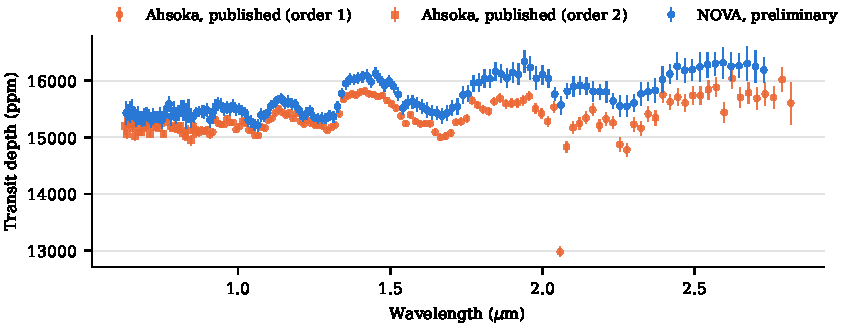
\includegraphics[width=\textwidth]{figures/nova_vs_published_wasp17_preliminary.pdf}
  \caption{Preliminary \nova{} transmission spectrum of the real WASP-17~b
  visit (blue) and the published Ahsoka spectrum of \citet{LouieEtAl2025} at
  a resolving power of 100 (orange; orders 1 and 2 shown separately). The
  \nova{} error bars are conditional on the fitted calibration products and
  geometry, and do not yet include the uncertainty from the planned ensemble.
  All points of both spectra are shown.}
  \label{fig:nova-real}
\end{figure*}

Figure~\ref{fig:nova-real} compares a preliminary NOVA spectrum of the real
WASP-17~b visit, from a reduction of 18 September 2026, with the published
Ahsoka spectrum of \citet{LouieEtAl2025}. This reduction used NOVA's own
white-light geometry, but it was fitted before the acceptance rule of
Section~\ref{sec:own-white} was written. Below about $1.8\,\mu\mathrm{m}$ the
two spectra show similar features, such as the water bands, but the NOVA
spectrum is deeper throughout. With the published spectrum interpolated to the
NOVA bins, NOVA is deeper by a median of about 230~ppm below
$1.6\,\mu\mathrm{m}$, 550~ppm between 1.8 and $2.3\,\mu\mathrm{m}$, and
490~ppm above $2.3\,\mu\mathrm{m}$.

Different geometry, limb-darkening and background treatments may all
contribute to this difference, and this comparison does not separate them. The
larger difference in the red matters most, because there the starlight is
faintest and the background matters most. The real data cannot decide whether
NOVA or the published reduction is closer to the truth. Separate injection
tests also found nonzero biases of NOVA, but these cannot be subtracted from
the difference on real data. This motivates the benchmark of the next two
sections, which is designed to measure the errors of each method when the
injected truth is known.
